\documentclass[12pt]{article}
 
\usepackage[margin=1in]{geometry} 
\usepackage{amsmath,amsthm,amssymb,bm}
\usepackage{graphicx}
 
\newcommand{\N}{\mathbb{N}}
\newcommand{\Z}{\mathbb{Z}}
 
\newenvironment{theorem}[2][Theorem]{\begin{trivlist}
\item[\hskip \labelsep {\bfseries #1}\hskip \labelsep {\bfseries #2.}]}{\end{trivlist}}
\newenvironment{lemma}[2][Lemma]{\begin{trivlist}
\item[\hskip \labelsep {\bfseries #1}\hskip \labelsep {\bfseries #2.}]}{\end{trivlist}}
\newenvironment{exercise}[2][Exercise]{\begin{trivlist}
\item[\hskip \labelsep {\bfseries #1}\hskip \labelsep {\bfseries #2.}]}{\end{trivlist}}
\newenvironment{reflection}[2][Reflection]{\begin{trivlist}
\item[\hskip \labelsep {\bfseries #1}\hskip \labelsep {\bfseries #2.}]}{\end{trivlist}}
\newenvironment{proposition}[2][Proposition]{\begin{trivlist}
\item[\hskip \labelsep {\bfseries #1}\hskip \labelsep {\bfseries #2.}]}{\end{trivlist}}
\newenvironment{corollary}[2][Corollary]{\begin{trivlist}
\item[\hskip \labelsep {\bfseries #1}\hskip \labelsep {\bfseries #2.}]}{\end{trivlist}}

\begin{document}
  
\title{Task 3. Relevance Vector Machine}
\author{Garoe Dorta-Perez\\
CM50246: Machine Learning and AI}
 
\maketitle
 
\section{Introduction}
 
SVM  are a popular choice in classification problems.
However they are inherently not probabilistic.
A technique that uses the same intuition is the Relevance Vector Machine.
It uses a full Bayesian approach with a prior that encourages sparseness.

\section{The problem}

First a dual model is used, previously we would model the data as a normal distribution.
Where $w$ is a one dimensional array with the world state, $x$ is the data point, $\phi$ are the parameters of a linear function of the data and $\sigma$ is the standard deviation.
We now apply a transformation on the parameters as shown in Equation ~\ref{eq:normal}, so $\phi$ is now a weighted sum over the observed data points, where $\psi$ is a vector with the weights.
If we are working with few data of high dimensionality, this sum is faster to calculate, as it has less terms, that the original linear dependency.

\begin{equation}
\label{eq:normal}
Pr(w_i|\mathbf{x}_i) = Norm_{x_i}[\phi^T \mathbf{x}_i, \sigma^2],
\end{equation}

\begin{equation}
\label{eq:dual}
\phi = \mathbf{X} \psi,
\end{equation}

Using the dual parameters $\psi$, we encourage sparsernes in the model by using the prior defined in Equation \ref{eq:prior}.
Where $I$ is the number of data points, $Stud$ is a Student's t-distribution with $\nu$ degrees of freedom and $\Gamma$ is the Gamma function.
Using a product of t-distributions produces the desired sparseness since the areas with higher probability density are in the origin and along the axis.

\begin{align}
\label{eq:prior}
Pr(\psi) &= \prod_{i = 1}^{I} Stud_{\psi_i} [0, 1, \nu],\\
&= \prod_{i=1}^I \frac{\Gamma \left( \frac{\nu + 1}{2} \right)}{ \sqrt{\nu \pi} \Gamma \left(\frac{\nu}{2} \right) } \left( 1 + \frac{\psi^2_i}{\nu} \right)^{- (\nu+1)/2},
\end{align}

A t-distribution is not conjugate to a Normal distribution, so there is no simple closed form solution for the posterior.
The solution will be to approximate the t-distributions by maximizing with respect to their hidden variables $h$, introduced in Equation \ref{eq:prHidden}, where $\mathbf{w}$ is a one dimensional array with the world state.
This leads to the marginal likelihood shown in Equation \ref{eq:likelihood}, where $\mathbf{I}$ is the identity matrix, $\mathbf{X}$ is a matrix with the data points and $\mathbf{H}$ is a matrix with all the hidden variables.

%Check this equation
\begin{equation}
\label{eq:prHidden}
Pr(\psi) = \prod_{i = 1}^{I} \int Norm_{\mathbf{w}}[0,1/h_i] Gam_{h_i}[\nu/2, \nu/2] dh_i,
\end{equation}

\begin{equation}
\label{eq:likelihood}
Pr(\mathbf{w}|\mathbf{X},\sigma^2) \approx \begin{array}{c}
		\\
      max \\
      \mathbf{ \mbox{\small H} }
    \end{array} \left[ Norm_{\mathbf{w}} \left[ \mathbf{0}, \mathbf{X}^T \mathbf{X} \mathbf{H}^{-1} \mathbf{X}^T \mathbf{X} + \sigma^2 \mathbf{I} \right] \prod_{d =1}^D Gam_{h_d} \left[ \nu /2, \nu/2 \right]  \right],
\end{equation}

The optimization is performed in three steps:
\begin{enumerate}
\item Optimize the marginal likelihood with respect to the hidden variables, using Equation \ref{eq:hiddenVar}.

\begin{equation}
\label{eq:hiddenVar}
h_i^{new} = \frac{1 - h_i \sum_{ii} + \nu}{\mu^2_i + \nu},
\end{equation}

\item Update $\boldsymbol{\mu}$ and $\mathbf{\Sigma}$, using Equation \ref{eq:muSigma}.

\begin{equation}
\label{eq:muSigma}
\begin{split}
\boldsymbol{\mu} &= \frac{1}{\sigma^2} \mathbf{A}^{-1} \mathbf{X}^T \mathbf{X} \mathbf{w},\\
\mathbf{\Sigma} &= \mathbf{A}^{-1},\\
\mathbf{A} &= \frac{1}{\sigma^2} \mathbf{X}^T \mathbf{X} \mathbf{X}^T \mathbf{X} + \mathbf{H},
\end{split}
\end{equation}

\item Optimize the marginal likelihood with respect to the variance parameter, using Equation \ref{eq:sigma}.
\end{enumerate}
 
\begin{equation}
\label{eq:sigma}
(\sigma^2)^{new} = \frac{1}{\mathbf{I} - \sum_i ( 1 - h_i \sum_{ii})}  \left( \mathbf{w} - \mathbf{X}^T \mathbf{X} \boldsymbol{\mu} \right)^T \left( \mathbf{w} - \mathbf{X}^T \mathbf{X} \boldsymbol{\mu} \right),
\end{equation}

After the training process, we only take the data points whose hidden variable $h_i$ is smaller than a threshold. Since a larger one means a small $\psi_i$, and hence no significance in the weighted sum.
In the implementation, we use a Gaussian kernel $k[x_i,x_j]$, as shown in Equation \ref{eq:kernel}, instead of calculating the inner products $\mathbf{X}^T \mathbf{X}$, where $\lambda$ controls the scale of the output.
This is more efficient than computing the inner product.
%and it has the advantage to correspond to computing infinite length $\mathbf{X}$.
%And using a nonlinear kernel is cool as well, dont remember how or why

\begin{equation}
\label{eq:kernel}
k[x_i, x_j] = exp \left[ - \frac{1}{2} \left( \frac{(x_i - x_j)^T (x_i - x_j)}{\lambda^2} \right) \right],
\end{equation}

Since our world states $\mathbf{w_i}$ are multivariate, a separate regressor is used for each dimension in  $\mathbf{w_i}$.
However the hidden variables matrix $\mathbf{H}$ is shared among all of them.

\section{Results}

In Figures \ref{fig:lambda} and \ref{fig:nu} we show results for a font data set.
The RVM is trained with pictures of \emph{n} in different fonts and their corresponding \emph{m} in the same font.
For testing, \emph{n} with new fonts are used.

\begin{figure}[h]
	\centering
	\begin{minipage}[t]{.45\textwidth}
		\centering
		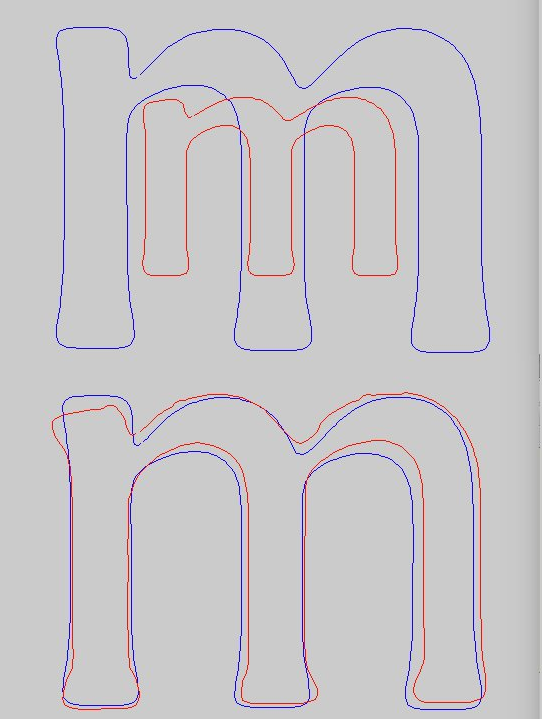
\includegraphics[scale=0.25]{images/lambda2_7}
		\caption{Blue is ground truth and red is RVM result. Top image corresponds to a kernel $\lambda=2$, bottom image has $\lambda=7$.}
		\label{fig:lambda}
	\end{minipage}\hfill
	\begin{minipage}[t]{.45\textwidth}
		\centering
		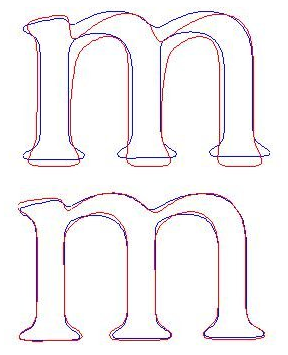
\includegraphics[scale=0.5]{images/nu1_0_01}
		\caption{Blue is ground truth and red is RVM result. Top image corresponds  $\nu=0.001$, bottom image has $\nu=1$}
		\label{fig:nu}
	\end{minipage}
\end{figure}

In Figure \ref{fig:lambda} we see the effects of changing the value of $\lambda$.
Since it controls the scale, we can see how the \emph{m} varies in size.
In Figure \ref{fig:nu} variations in $\nu$ are shown.
Smaller $\nu$ encourages more sparsity, and so less relevance vectors been used.
For the top image 5 relevance vectors are used, while for the bottom one 10 vectors are used.
Less vectors means a more general and sparse model used. 
However the error in the prediction increases as we take fewer relevance vectors. 

%Talk about linearity and overfitting

\end{document}